%! Author = matteomagnini
%! Date = 03/03/26

% Preamble
\documentclass[11pt]{article}

% Packages
\usepackage{amsmath}
\usepackage{amssymb}
\usepackage{tikz}
\usepackage{hyperref}
\usetikzlibrary{positioning}

\title{
    Intelligent Systems 2\\
    Tutorial week 3: Modal Logic
}

\author{
    Matteo Magnini\\
    \href{mailto:matteo.magnini@uni.lu}{matteo.magnini@uni.lu}
}

\date{
    5 March, 2026
}

% Document
\begin{document}

    \maketitle

    \section{Exercises}\label{sec:exercises}

    \subsection{Exercise 1: Kripke Structure Analysis}\label{subsec:exercise-1}

    Consider the following Kripke structure $M = (S, R, V)$:

    \begin{center}
        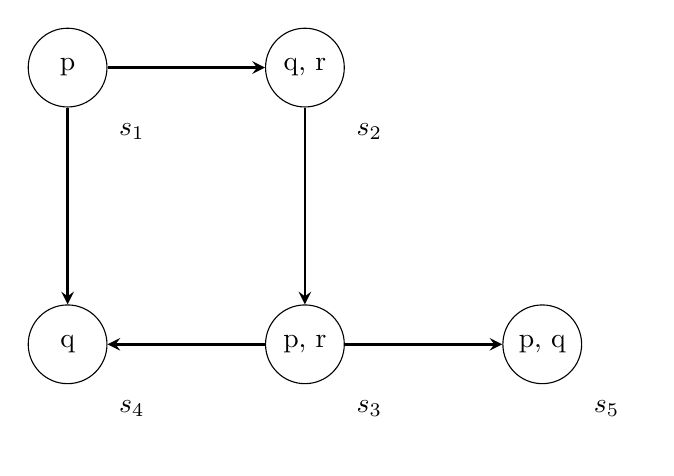
\begin{tikzpicture}[
            node distance=2.5cm and 2cm,
            every node/.style={draw,circle, minimum size=1cm},
            >=stealth
        ]
            % Nodes with predicates inside
            \node (s1) {p};
            \node[right=of s1] (s2) {q, r};
            \node[below=of s2] (s3) {p, r};
            \node[below=of s1] (s4) {q};
            \node[right=of s3] (s5) {p, q};

            % State labels (pedice)
            \node[below right=0.1cm and 0.1cm of s1, draw=none] {$s_1$};
            \node[below right=0.1cm and 0.1cm of s2, draw=none] {$s_2$};
            \node[below right=0.1cm and 0.1cm of s3, draw=none] {$s_3$};
            \node[below right=0.1cm and 0.1cm of s4, draw=none] {$s_4$};
            \node[below right=0.1cm and 0.1cm of s5, draw=none] {$s_5$};

            % Edges
            \draw[->, line width=1pt] (s1) -- (s2);
            \draw[->, line width=1pt] (s1) -- (s4);
            \draw[->, line width=1pt] (s2) -- (s3);
            \draw[->, line width=1pt] (s3) -- (s4);
            \draw[->, line width=1pt] (s3) -- (s5);
        \end{tikzpicture}
    \end{center}

    Which of the following statements are true?
    Explain your answer.
    \begin{enumerate}
        \item[(a)] $M, s_1 \models p$
        \item[(b)] $M, s_1 \models \Box q$
        \item[(c)] $M, s_2 \models q \wedge \Box q$
        \item[(d)] $M, s_3 \models \Box q \wedge \Diamond r$
        \item[(e)] $M \models q \lor \Diamond q$
    \end{enumerate}

    \subsection{Exercise 2}\label{subsec:exercise-2}

    Show that each of the following formulas is not a tautology.
    \begin{enumerate}
        \item[(a)] $\Box \bot$
        \item[(b)] $\Diamond p \rightarrow \Box p$
        \item[(c)] $p \rightarrow \Box \Diamond p$
        \item[(d)] $\Diamond \Box p \rightarrow \Box \Diamond p$
    \end{enumerate}

    \subsection{Exercise 3}\label{subsec:exercise-3}

    Is it possible to define the semantics of $\Box$ and $\Diamond$ by truth tables?
    In order to answer that question, consider the following constraints for an epistemic interpretation of the $\Box$ operator (read $\Box A$ as ``A is known''):
    \begin{itemize}
        \item We want $\Box A \rightarrow A$ to be valid \\
        (``If something is known, then it is true.'')
        \item $A \rightarrow \Box A$ should not be valid \\
        (``Not all true things are indeed known.'')
        \item $\neg \Box A$ should not be valid \\
        (``There are things that are not known.'')
    \end{itemize}
    \textbf{Hint:} Try to construct a truth table for $\Box$ that satisfies these constraints.

    \subsection{Exercise 4}
    \label{subsec:exercise-4}

    Show that the satisfaction of a formula $\varphi$ within a given model is only dependent on the valuation $V$ of the propositional symbols occurring in $\varphi$. In particular, assume that $V$ and $V'$ are two valuations on the frame $(W, R)$ such that $V(p) = V'(p)$ for all symbols $p$ in $\varphi$. Show that
    \[
    (W, R, V) \models \varphi \quad \text{if and only if} \quad (W, R, V') \models \varphi.
    \]
    \textbf{Hint:} Prove this by induction on the number of connectives in $\varphi$.

\end{document}